\section{Two-component regularization for singular sources}
\label{2_comp_reg}
To avoid the difficulty due to the source term and the work for solving the Laplace equation we consider a two component regularization proposed by Cai, Wang and Zhao \cite{Cai2009}. For this regularization the electrostatic potential $\phi$ has been considered as the addition of the coulmb component $\phi_c$ and the reaction field component $\phi_{RF}$ as $\phi= \phi_c +\phi_{RF}$. Here $\phi_c$ satisfies the following Poission's equation, 
\begin{equation}
	\begin{cases}
		-\epsilon^- \Delta\phi_C(r) = \rho(r) \text{   in   }\mathbb{R}^3 \label{rho_eq} \\
		\text{      }\phi_C(r)= 0. \text{   as  } |r| \rightarrow \infty
	\end{cases}
\end{equation}
which gives us the analytical solution as the Green's function $G$ for $\phi_C$ as,
\begin{equation}
	G(r) = \frac{e_c^2}{k_B T } \sum_{i=1}^{N_c} \frac{q_i }{\epsilon^{-}|r-r_i|} \label{Green} %\text{ where } C = \frac{e_c^2}{k_B T }
\end{equation}
	
%	Now the non-linear PBE from (\ref{pbe}) can be rewritten as,
%	
%	  \begin{eqnarray}
%				-\nabla.(\epsilon\nabla (\phi_C(\textbf{r})))-\nabla.(\epsilon\nabla (\phi_{RF}(\textbf{r})))+\bar\kappa^2(\textbf{r}) \sinh (\phi_C(\textbf{r})+\phi_{RF}(\textbf{r}))&=&\rho(\textbf{r}), \text{ in } \Omega \label{pbe_reg} %\\
%						%\left[\phi \right]_\Gamma = 0 \textnormal{ and } \left[\epsilon\phi_n\right]_\Gamma = 0 
%	\end{eqnarray}
%	
%	The reaction field components can be physically interpreted as the electrostatic field generated by the charges induced by changes of dielectric constant of the  solvent around the solute from $\epsilon^-$ to $\epsilon^+$ \cite{Cai2009}. Now substituting (\ref{rho}) into (\ref{pbe_reg}) we have,
%	\begin{eqnarray}
%	-\nabla(\epsilon^+ \phi_{RF}(\textbf{r})) +\bar\kappa^2 \sinh(\phi_C(\textbf{r})+\phi_{RF}(\textbf{r}))&=& 0 \text{ in } \Omega^- \cup \Omega^+	
%	\end{eqnarray}
%	More explicitly $\phi_{RF}$ satisfies the following elliptic interface problem \cite{Chen2007}, 
%\begin{eqnarray}
%		-\nabla.(\epsilon^- \nabla  \phi_{RF}) &=& 0 \text{ in } \Omega^-\\  
%		-\nabla(\epsilon^+ \phi_{RF}) +\bar\kappa^2 \sinh(\phi_C+\phi_{RF})&=& 0 \text{ in } \Omega^+\\
%		\left[\phi_{RF}\right] &=& 0 \text{ on } \Gamma \\
%		\left[\epsilon\frac{\partial \phi_{RF}}{\partial n}\right]&=& (\epsilon^+-\epsilon^- ) \frac{\partial G}{\partial n} \text{ on } \Gamma\\
%		\phi_{RF}&=& \phi_b-G \text{ on } \partial \Omega \label{rf_sys}
%	\end{eqnarray} 
%	
%So now there is no singular term on the right hand side but we still have several numerical difficulties. In \cite{Holst2010} its been reported that $\phi_C$ and $\phi_{RF}$ have different signs and their magnitude is much larger than that of $\phi$. Here  a relatively small error in $\phi_{RF}$ will produce a relatively larger error in $\phi$ given that the $phi_C$ is analytically calculated. Sometimes this amplifying factor can be as large as $(\epsilon^+/\epsilon^- - 1 )$ \cite{Holst2010}. In our case this factor is about $79$ by taking $\epsilon^+=80$ and $\epsilon^-=1$. Another problem is, the calculation of $\phi_C$ is necessary for all N grid points in $\Omega^+$ at a computational cost $O(N^2)$ which is very expensive for large $N$. 
%
Then Luo and his collaborators \cite{Cai2009} proposed to solve for the original solution $\phi$ in $\Omega^+$ instead of the reaction component $\phi_{RF}$. Now to make the required adjustments to fit this regularization approach \cite{Cai2009} with finite difference and finite element method Zhao and Geng \cite{Geng2017a} proposed a new elliptic problem with discontinuous function flux jumps for the two-component regularization. In particular they defined the regularized potential as,  
	
\begin{eqnarray}
	\tilde{ \phi} &=& \begin{cases}
	\phi_{RF} \text{ in } \Omega^-\\
	\phi_C + \phi_{RF} \text{ in } \Omega^+\\
	\end{cases}
\end{eqnarray}
 
The jump conditions for $\tilde\phi $ were derived from $\phi$ and the definition $\phi=\phi_C+\phi_{RF}$ as,

\begin{eqnarray}
\phi^+=\phi^-_{RF}+\phi^-_C,\text{  and  } \epsilon^+ \frac{\partial \phi^+}{\partial n}=\epsilon^- \frac{\partial \phi^-_{RF}}{\partial n}+\epsilon^- \frac{\partial \phi^-_C}{\partial n} \text{ on } \Gamma
\end{eqnarray}

Thus, the regularized PB equation of $\tilde \phi$ with corresponding interface and boundary conditions are given as. 
\begin{eqnarray}
	-\nabla.(\epsilon^- \nabla \tilde{ \phi}) &=& 0 \text{ in } \Omega^-\\ \label{phitilde1}
	-\nabla.(\epsilon^+ \nabla \tilde{ \phi}) +\bar\kappa^2 \sinh(\tilde{ \phi})&=& 0 \text{ in } \Omega^+\\\label{phitilde2}
	\left[\tilde{ \phi}\right] &=& G \text{ on } \Gamma \\ \label{phitilde3}
	\left[\epsilon\frac{\partial \tilde{ \phi}}{\partial n}\right]&=& \epsilon^-  \frac{\partial G}{\partial n} \text{ on } \Gamma\\\label{phitilde4}
	\tilde{\phi} &=& \phi_b \text{ on } \partial \Omega \label{phitilde5}
\end{eqnarray}	
	


Now from (\ref{phitilde1}) and (\ref{phitilde5}) we can summarize that, 

\begin{eqnarray}
	-\nabla . (\epsilon \nabla \tilde{ \phi}) +\bar\kappa^2 \sinh(\tilde{ \phi})&=& 0 \text{ in } \Omega^-\cup\Omega^+\label{RPB}
\end{eqnarray}
	 
where $\tilde \phi$	 satisfies the PB equation without the source term. Then Zhao and Geng \cite{Geng2017a} proposed to numerically solve the regularized PB interface problem (RPB) given in (\ref{phitilde1})-(\ref{phitilde5}) and to finally recover the original solution as $\phi= \tilde\phi $ in $\Omega^+$ and $\phi = \tilde \phi + G $ in $\Omega^-$, Where the Green's function $G$ is analytically given.
%%%%%%%%%%%%%%%%%%%%%%%%%%%%%%%%%%%%%%%%%%%%%%%%%%%%%%%%%%%%%%%%%%%%%%%%%%%%%


\section{Pseudo-transient continuation approach for the PBE}

As the pseudo-transient continuation approach, an indirect method discussed in \cite{zhao_pseudo-time-coupled_2011,Sayyed-Ahmad2004,shestakov_solution_2002} introduced a pseudo-time derivative to solve the PB equation as,  

\begin{eqnarray}
	 	\frac{\partial u}{\partial t} &=& \nabla.(\epsilon \nabla u)-\bar\kappa^2 \sinh(u) \text{ in } \Omega^- \cup \Omega^+ \label{tdrpb} \\
	 	  \left[u\right]&=& G,\text{ and } \left[\epsilon\frac{\partial u}{\partial n}\right]= \epsilon^-  \frac{\partial G}{\partial n} \text{ on } \Gamma\\ \label{jump}
	 	  u&=&\phi_b \text{ on } \partial \Omega
	\end{eqnarray}

Here the time independent regularized PB equation in (\ref{RPB}) has been converted in to a time dependent regularized PB (TDRPB) in (\ref{tdrpb}). Our goal is to first specify the initial condition, which could be the electrostatic potential solved from a linearized PB \cite{zhao_pseudo-time-coupled_2011} equation or trivially $u = 0$ and then numerically integrate (\ref{tdrpb}) for a sufficiently long period to get the steady state solution as the solution of the original regularized PB (\ref{RPB}). Here the sign on the right hand side of eq. (\ref{tdrpb}) has been considered as the reverse of the eq.(\ref{RPB}) to ensure the numerical stability. 

But, there are difficulties in the numerical integration of the TDRPB equation (\ref{tdrpb}) because of the requirement of long time integration, when explicit time stepping methods are usually not efficient \cite{Sayyed-Ahmad2004},\cite{shestakov_solution_2002},\cite{zhao_pseudo-time-coupled_2011}, \cite{zhao_operator_2014}. Hence we are employing a semi-implicit time splitting method \cite{Sayyed-Ahmad2004},\cite{shestakov_solution_2002} which have been commonly used to solve the TDPB in the literature. 

Let us consider a uniform mesh with a grid spacing $h$ in all $x,y$ and $z$ directions having $N_x,N_y$ and $N_z$ as the number of the grid points in each direction. We assume the vector $U^n={\tilde\phi^n_{ijk}}$ for $i=1,...., N_x,j=1,...,N_y,k=1,...N_z$ denote all the nodal values of $\tilde\phi$ at the time level $t_n$. We will develop several schemes for updating $U^n$ at time level $t_n$ to $U^{n+1}$ at time level $t_{n+1}=t_n+ \Delta t $. In this time dependent RPB we will consider only $U$ as time dependent, while all other functions in (\ref{tdrpb}) i.e. $\epsilon$ and $\bar\kappa^2 $ are time independent. 

%%%%%%%%%%%%%%%%%%%%%%%%%%%%%%%%%%%%%%%%%%%%%%%%%%%%%%%%%%%%%%%%%%%%%%%%%%%%%

\section{ADI method with Implicit-Euler method (GFM-ADI)}
\label{sec:GFM-ADI}

In this scheme at each time step from $t_n$ to $t_{n+1}$, the time dependent equation TDRPB in  (\ref{tdrpb}) will be solved by a first order time splitting in two stages, 
\begin{eqnarray}
  \frac{\partial w}{\partial t}&=& -\bar\kappa^2 \sinh(w) \text{ with } W^n=U^n\text{ and } t \in \left[t_n,t_{n+1}\right]\label{non_linear_ADI}\\
 \frac{\partial v}{\partial t}&=&  \nabla . (\epsilon\nabla v) \text{ with } V^n=W^{n+1}\text{ and } t \in \left[t_n,t_{n+1}\right]	 \label{diffusion_ADI}
\end{eqnarray}  
Altogether we have $U^{n+1}=V^{n+1}$. And for $ \frac{\partial w}{\partial t}= -\bar\kappa^2 \sinh(w)$ we have the analytical solution as, 	
	\begin{eqnarray}	
W^{n+1}= \ln \left( \frac{\cosh(\frac{1}{2}\bar\kappa^2\Delta t)+\exp(-W^n)\sinh(\frac{1}{2}\bar\kappa^2\Delta t)}{\exp(-W^n)\cosh(\frac{1}{2}\bar\kappa^2\Delta t)+\sinh(\frac{1}{2}\bar\kappa^2\Delta t)}\right)\label{anal_sol}
\end{eqnarray}
Which will help us to avoid to the difficulty due to the non-linear term with $\sinh(.)$ in (\ref{pbe}). Here the right hand side of equation (\ref{anal_sol}) is just a function of $W$ and $\Delta t$ which allows us to rewrite the equation $(\ref{anal_sol})$ as $W^{n+1}=F(W^n,\Delta t)$ to facilitate the following discussion. 
For the temporal discretization of the equation (\ref{diffusion_ADI}) we have used Backward-Euler integration in time to get, 
\begin{eqnarray}
	v_{i,j,k}^{n+1} &=v_{i,j,k}^{n}+\Delta t \left(\delta_x^2+\delta_y^2+\delta_z^2\right)v_{i,j,k}^{n+1} \label{imp-eu}
\end{eqnarray}	

 Where $\delta_x^2,\delta_y^2$ and $\delta_z^2$ are the central finite difference operators defined in (\ref{dif_opz}) for the $x,y$ and $z$ directions, respectively with $\epsilon_{i,j,k}= \displaystyle\begin{cases}
	\epsilon^- \text{ if } x_{i,j,k}\in\Omega^- \cup \Gamma \\
	\epsilon^+ \text{ if } x_{i,j,k}\in\Omega^+\\
	\end{cases}$.

 \begin{eqnarray}
 \begin{aligned}
	\delta_x^2\left(v_{i,j,k}^n\right)&= \frac{\epsilon_{i,j,k}}{h^2} \left(v_{i-1,j,k}^n-2v_{i,j,k}^n+v_{i+1,j,k}^n\right) \\ \label{dif_opx}
	\delta_y^2\left(v_{i,j,k}^n\right)&= \frac{\epsilon_{i,j,k}}{h^2} \left(v_{i,j-1,k}^n-2v_{i,j,k}^n+v_{i,j+1,k}^n\right)\\ %\label{dif_opy}
	\delta_z^2\left(v_{i,j,k}^n\right)&= \frac{\epsilon_{i,j,k}}{h^2} \left(v_{i,j,k-1}^n-2v_{i,j,k}^n+v_{i,j,k+1}^n\right) \label{dif_opz}
\end{aligned}
\end{eqnarray}

%\end{equation}
%on the points far away from the interface $\Gamma$ which are defined as regulars nodes.
But at the  points near the interface the central difference operators defined in (\ref{dif_opx})-(\ref{dif_opz}) will not be applicable. These points are defined as the irregular points where at-least one of its adjacent points is on the other side of the boundary. On the irregular points one of the three point stencils for $\delta_x^2,\delta_y^2$ and $\delta_z^2$  will be on the other side of the interface where the information about the function $v$ is not available. A non-standard finite difference formula is necessary on the irregular points to discretize $\delta_x^2,\delta_y^2$ and $\delta_z^2$.  In this regard a modified version of the Ghost Fluid Method has been proposed in Section \ref{new_gfm} using the fictitious points (or ghost points) and the jump conditions in (\ref{jump}) rigorously.

\begin{figure}[!ht]
	\centering
	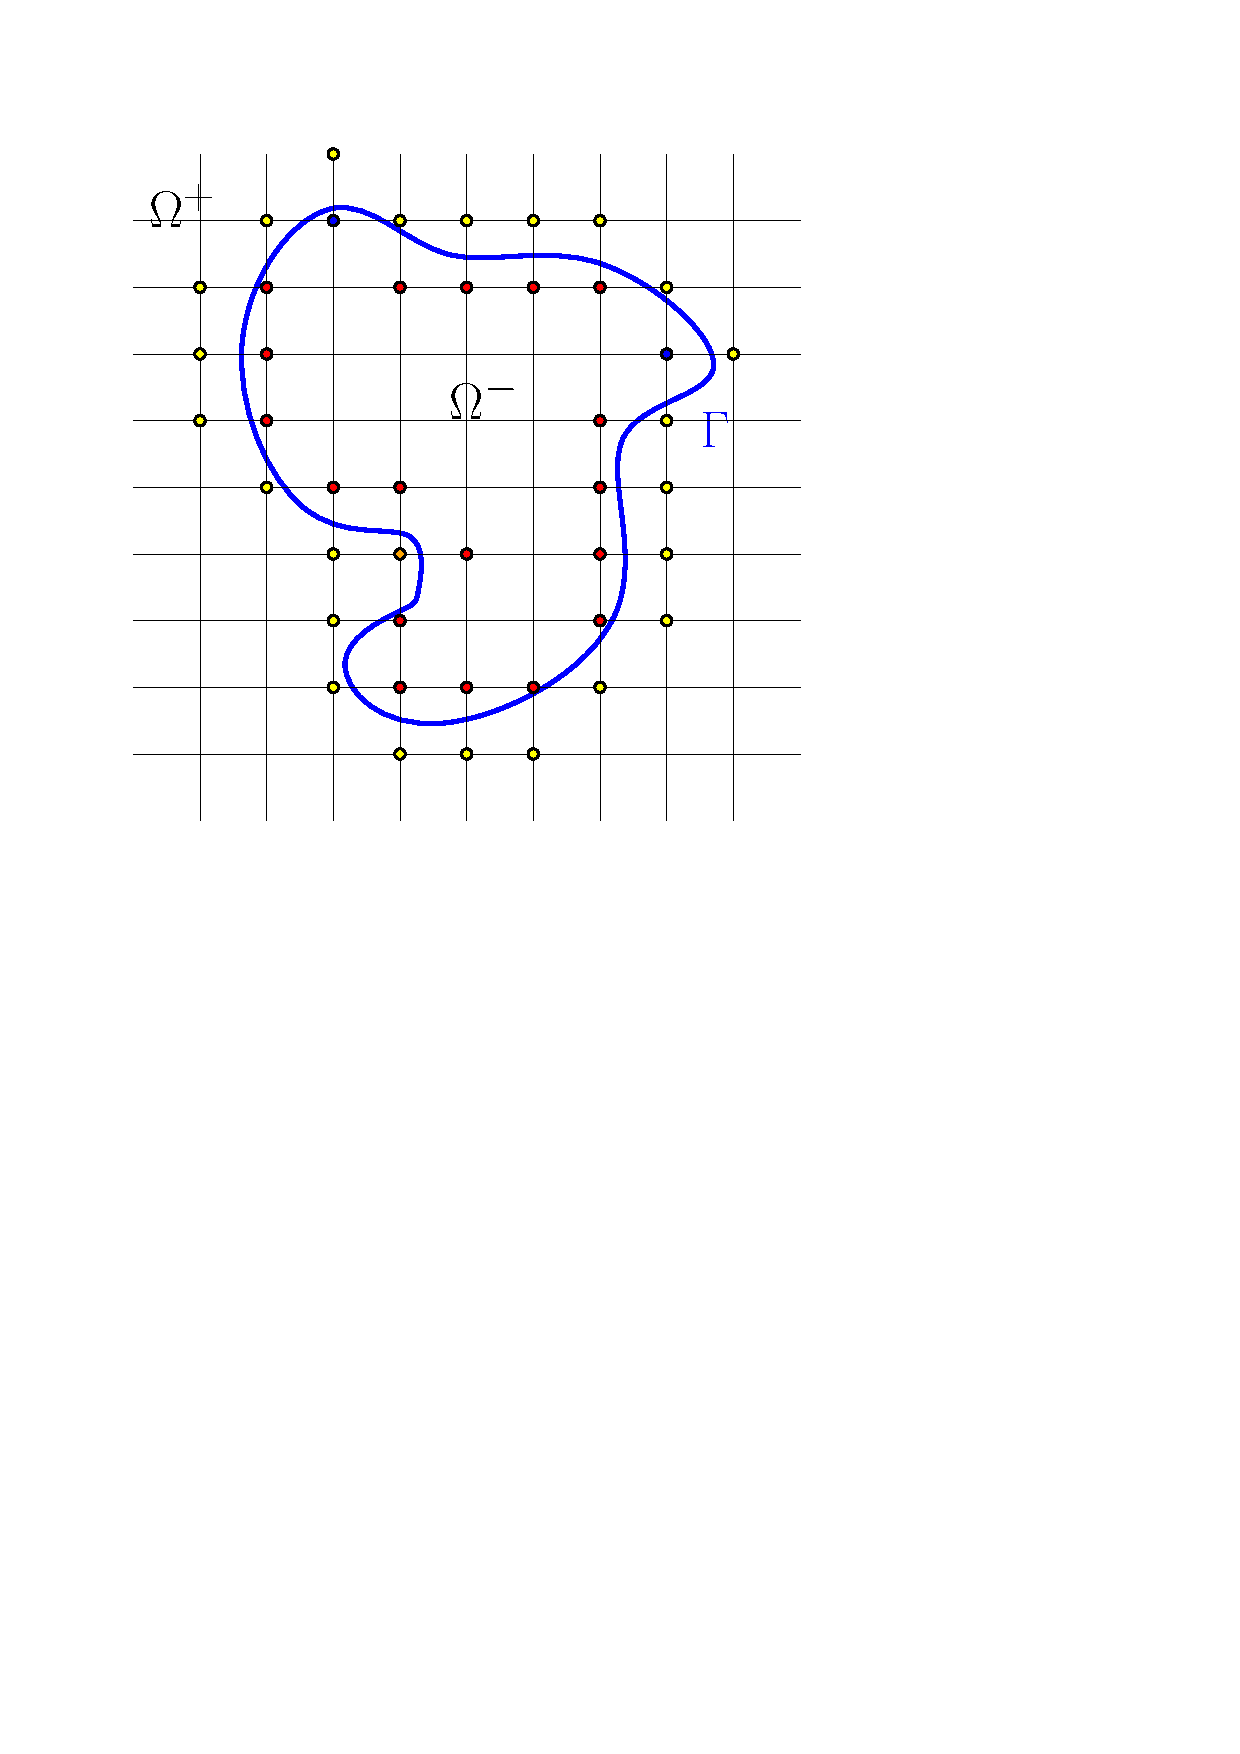
\includegraphics[scale = .7]{PBE1_grid.pdf}
	\caption{Irregular grid points marked as colored disks with blue and orange color for corner points.}
	\label{fig_irgpoints}
\end{figure}

Then a first order Douglas-Rachford type ADI scheme has been used to decompose the diffusion equation (\ref{imp-eu}) in $x,y$ and $z$ directions as,  
\begin{eqnarray}
%\begin{aligned}
		\left(1- \Delta t \delta_x^2\right)v_{i,j,k}^{*}&=&\left[1+ \Delta t \left(\delta_y^2+\delta_z^2 \right)\right]v_{i,j,k}^{n}\label{GFM-ADI}\\
		\left(1-\Delta t \delta_y^2\right)v_{i,j,k}^{**}&=&v_{i,j,k}^{*}- \Delta t \delta_y^2\left(v_{i,j,k}^{n}\right)\label{GFM-ADI2}\\
		\left(1- \Delta t \delta_z^2\right)v_{i,j,k}^{n+1}&=&v_{i,j,k}^{**}- \Delta t \delta_z^2\left(v_{i,j,k}^{n}\right)\label{GFM-ADI3}
%\end{aligned}		\label{1dadi}
\end{eqnarray} 
Where $v^*$ and $v^{**}$ are two intermediate values to create three tridiagonal one dimensional system. Here, the three dimensional linear algebraic system in equation (\ref{imp-eu}) has been decomposed into several one dimensional linear algebraic systems in (\ref{GFM-ADI}), (\ref{GFM-ADI2}) and (\ref{GFM-ADI3}).  Each one these equations has a tridiagonal structure. These three tridiagonal systems are much more efficient to solve than one non-structured system in (\ref{imp-eu}). Then by eliminating $v^*_{i,j,k}$ and $v^{**}_{i,j,k}$ and solving for $v^{n+1}_{i,j,k}$ in (\ref{imp-eu}) we get,
\begin{eqnarray}
\begin{aligned}
	v^{n+1}_{i,j,k}&=v^n_{i,j,k}+ \Delta t \left(\delta_x^2+\delta_y^2+\delta_z^2\right) v^{n+1}_{i,j,k} -\Delta t^2 \left(\delta_x^2\delta_y^2+\delta_x^2\delta_y^2+\delta_z^2\delta_y^2\right)(v^{n+1}_{i,j,k}-v^{n}_{i,j,k})\\
	&+ \Delta t^3 \delta_x^2\delta_y^2\delta_z^2(v^{n+1}_{i,j,k}-v^{n}_{i,j,k}) \label{adi_tailor}
	\end{aligned}
\end{eqnarray}
Hence the Douglas-Rachford scheme (\ref{imp-eu}) is a higher order perturbation of the Implicit-Euler method. Since both (\ref{non_linear_ADI}) and (\ref{diffusion_ADI}) are first order in time this proposed ADI-IE-GFM scheme is of first order accuracy in time. As the boundary conditions the same Dirichlet boundary boundary values are assumed for $v$, $v^*$ and  $v^{**}$ for $u$. The entire time integration here is fully implicit. 

%%%%%%%%%%%%%%%%%%%%%%%%%%%%%%%%%%%%%%%%%%%%%%%%%%%%%%%%%%%%%%%%%%%%%%%%%%%%%

\section{LOD with Crank-Nicolson method(GFM-LODCN)}\label{GFM-LODCN}
In this scheme at each time step from $t_n$ to $t_{n+1}$, the time dependent non-linear equation TDPBE will be solved by a second order time splitting methods in three stages \cite{Yu2005},
\begin{eqnarray}
  \frac{\partial w}{\partial t}&=& -\frac{1}{2}\bar\kappa^2 \sinh(w) \text{ with } W^n=U^n\text{ and } t \in \left[t_n,t_{n+1}\right]\label{non_linear1_LOD-CN}\\
 \frac{\partial v}{\partial t}&=&  \nabla . (\epsilon\nabla v) \text{    with } V^n=W^{n+1}\text{ and } t \in \left[t_n,t_{n+1}\right]	 \label{diffusion_LOD-CN}\\
 \frac{\partial \tilde{w}}{\partial t}&=& -\frac{1}{2}\bar\kappa^2 \sinh( \tilde{w}) \text{ with } \tilde{W}^n=V^{n+1}\text{ and } t \in \left[t_n,t_{n+1}\right]\label{non_linear2_LOD-CN}
\end{eqnarray}
We then have $U^{n+1}=\tilde{W}^{n+1}$. As in the subsection \ref{GFM-ADI_sec} we will use an analytical integration in the first and the last stage of this scheme. Symbolically, we have $W^{n+1}=F(W^n,\frac{\Delta t}{2})$ and $\tilde{W}^{n+1}=F(\tilde{W}^n,\frac{\Delta t}{2})$, where $F$ is defined as in Eq.(\ref{anal_sol}).\\
Then we have proposed another multiplicative operator splitting scheme called as Locally One Dimensional (LOD) scheme to solve the diffusion equation (\ref{diffusion_LOD-CN}). This types of fractional step methods were first developed by Russian mathematicians in \cite{Yakonov_1963}, \cite{Yanenko_1963}, \cite{Yanenko_1967}. The discretization of (\ref{diffusion_LOD-CN}) using Crank-Nicolson integration in time and central differencing in space results in, 
\begin{eqnarray}
	\left(1-\frac{\Delta t}{2}(\delta^2_x+\delta^2_y+\delta^2_z)\right)v_{i,j,k}^{n+1}=\left(1+\frac{\Delta t}{2}(\delta^2_x+\delta^2_y+\delta^2_z)\right)v_{i,j,k}^n
\end{eqnarray}
Which can be decomposed in to $x,y$ and $z$ directions to give a LOD scheme for (\ref{diffusion_LOD-CN}),
\begin{eqnarray}
	\begin{aligned}
	\left(1-\frac{\Delta t}{2}\delta_x^2\right)v^*_{i,j,k}&=\left(1+\frac{\Delta t}{2}\delta_x^2\right)v^n_{i,j,k}\\
	\left(1-\frac{\Delta t}{2}\delta_y^2\right)v^{**}_{i,j,k}&=\left(1+\frac{\Delta t}{2}\delta_y^2\right)v^*_{i,j,k}\\
	\left(1-\frac{\Delta t}{2}\delta_z^2\right)v^{n+1}_{i,j,k}&=\left(1+\frac{\Delta t}{2}\delta_z^2\right)v^{**}_{i,j,k}\label{LODCN_eq}
	\end{aligned}
\end{eqnarray}

Similarly as the GFM-ADI scheme described in subsection \ref{GFM-ADI_sec} the tridiagonal systems in (\ref{LODCN_eq}) can be efficiently solved by the Thomas algorithm. 

%%%%%%%%%%%%%%%%%%%%%%%%%%%%%%%%%%%%%%%%%%%%%%%%%%%%%%%%%%%%%%%%%%%%%%%%%%%%%


\section{LOD with Implicit-Euler method (GFM-LODIE)}

For this scheme at each time step from $t_n$ to $t_{n+1}$, the time dependent equation TDRPB in  (\ref{tdrpb}) will be solved by the first order time splitting  similar to the GFM-ADI scheme described in the subsection \ref{GFM-ADI_sec} in two stages. To follow the same steps in the first stage Eq. (\ref{non_linear_ADI}) will be solved analytically by the function $W^{n+1}=F(W^n,\Delta t)$ in Eq. (\ref{anal_sol}) and in the second stage for the temporal discretization of the Eq.  (\ref{diffusion_ADI}) we have used Implicit Euler method to get Eq.(\ref{imp-eu}). 
 
 Then we have applied the LOD scheme described in the subsection \ref{GFM-LODCN} to decompose Eq. (\ref{imp-eu})  in to $x,y$ and $z$ direction as, 
 
\begin{eqnarray}
\begin{aligned}
		(1-\Delta t \delta_x^2)v^*_{i,j,k} &= v^n_{i,j,k}\\
		(1-\Delta t \delta_y^2)v^{**}_{i,j,k} &= v^*_{i,j,k}\\
		(1-\Delta t \delta_z^2)v^{n+1}_{i,j,k} &= v^{**}_{i,j,k}\\
	\end{aligned}
\end{eqnarray}	
Which will solved individually by the Thomas Algorithm like the previous subsections. 
% At each time step from $t_n$ to $t_{n+1}$ the diffusion equation (\ref{non_linear_ADI}) and (\ref{diffusion_ADI}) in fi
%
%\begin{eqnarray}
%\begin{aligned}
% \frac{\partial w}{\partial t}=& -\bar\kappa^2 \sinh(w) \text{ with } W^n=U^n\text{ and } t \in \left[t_n,t_{n+1}\right] \\
%   \frac{\partial v}{\partial t}=& \frac{\partial}{\partial x}\left(\epsilon \frac{\partial v}{\partial x}\right ), \text{ with } V^n=W^{n+1}\text{ and } t \in \left[t_n,t_{n+1}\right]\\	
%     \frac{\partial p}{\partial t}=& \frac{\partial}{\partial y}\left(\epsilon \frac{\partial p}{\partial y}\right ), \text{ with } P^n=V^{n+1}\text{ and } t \in \left[t_n,t_{n+1}\right]\\
%      \frac{\partial q}{\partial t}=& \frac{\partial}{\partial z}\left(\epsilon \frac{\partial q}{\partial z}\right ), \text{ with } Q^n=P^{n+1}\text{ and } t \in \left[t_n,t_{n+1}\right]	
%%       \frac{\partial s}{\partial t}&=& 0, \text{ with } S^n=Q^{n+1}\text{ and } t \in \left[t_n,t_{n+1}\right]
%\end{aligned}	
%\end{eqnarray}
%And finally $U^{n+1}=P^{n+1}$. Which will give us the following systems to solve,
%	\begin{eqnarray}
%	\begin{aligned}
%		w_{i,j,k} =& \ln \left[ \frac{\cosh(\frac{1}{2}\bar\kappa^2\Delta t)+\exp(-u^n_{i,j,k})\sinh(\frac{1}{2}\bar\kappa^2\Delta t)}{\exp(-u^n_{i,j,k})\cosh(\frac{1}{2}\bar\kappa^2\Delta t)+\sinh(\frac{1}{2}\bar\kappa^2\Delta t)}\right]\\
%		(1-\Delta t \delta_x^2)v_{i,j,k} =& w_{i,j,k}\\
%		(1-\Delta t \delta_y^2)p_{i,j,k} =& v_{i,j,k}\\
%		(1-\Delta t \delta_z^2)q_{i,j,k} =& p_{i,j,k}\\
%		u^{n+1}_{i,j,k} =& q_{i,j,k} \label{lod_split}
%		\end{aligned}
%	\end{eqnarray}	
%\subsection{Spatial Discritization}
%		We will approximate the the spatial derivatives in (\ref{dif2}), (\ref{1dadi}), (\ref{adi_tailor}) and (\ref{lod_split}) by the finite difference operators $\delta_{xx}, \delta_{yy}$ and $\delta_{zz}$ by the standard central finite difference formula as,  
%		\begin{eqnarray}
%			\begin{aligned}
%				\frac{\partial^2}{\partial x^2}\left(u_{i,j,k}^n\right)& \approx \delta_{xx}\left(u_{i,j,k}^n\right):= \frac{1}{\Delta x^2} \left(u_{i-1,j,k}^n-2u_{i,j,k}^n+u_{i+1,j,k}^n\right)\\
%				\frac{\partial^2}{\partial y^2}\left(u_{i,j,k}^n\right)& \approx \delta_{yy}\left(u_{i,j,k}^n\right):= \frac{1}{\Delta y^2} \left(u_{i,j-1,k}^n-2u_{i,j,k}^n+u_{i,j+1,k}^n\right)\\
%				\frac{\partial^2}{\partial z^2}\left(u_{i,j,k}^n\right)& \approx \delta_{zz}\left(u_{i,j,k}^n\right):= \frac{1}{\Delta z^2} \left(u_{i,j,k-1}^n-2u_{i,j,k}^n+u_{i,j,k+1}^n\right)\label{space_discrit}
%			\end{aligned}
%		\end{eqnarray}
%	 
